
\stilian{Here, we examine numerically the applicability of the asymptotic boundaries 
\eqref{eq:strong-classification-boundary} for finite $p$.  We consider independent errors and several popular models of the marginal distribution.  Numerical experiments for dependent errors will be deferred to Chapter \ref{chap:URS}.}{\fbox{check}}

To demonstrate the phase transition phenomenon under different error tail densities, we simulate from the additive error model \eqref{eq:model-additive} with
\begin{itemize}
    \item Gaussian errors, where the density is given by
    $f(x) = \frac{1}{\sqrt{2\pi}}\exp{\left\{-x^2/2\right\}}$.
    \item Laplace errors, where the density is given by $f(x) = \frac{1}{2}\exp{\left\{-\left|x\right|\right\}}$.
    \item Generalized Gaussian $\nu=1/2$, with density
    $f(x) = \frac{1}{2}\exp{\big\{-2\left|x\right|^{1/2}\big\}}$.
\end{itemize}
The sparsity and signal size of the sparse mean vector are parametrized as in equations \eqref{eq:sparsity-parametrized} and \eqref{eq:signal-size-parametrized}, respectively.
The support set $S$ is estimated with 
$\widetilde{S} = \left\{i:x(i)>\sqrt{2\log{p}}\right\}$ 
under the Gaussian errors, 
$\widetilde{S} = \left\{i:x(i)>\log{p} + (\log{\log{p}})/2\right\}$ 
under the Laplace errors, and with
$\widetilde{S} = \{i:x(i)> \frac{1}{4}\left(W\left(-c/(ep\log{p})\right) + 1\right)^2\}$
under the generalized Gaussian ($\nu = 1/2$) errors. Here $W$ is the Lambert W function, i.e., $W=f^{-1}$ where $f(x)=x\exp{(x)}$.
The choices of thresholds correspond to Bonferroni's procedures with FWER decreasing at a rate of 
${\cal O}(1/\sqrt{\log{p}})$, therefore satisfying the assumptions in Theorem \ref{thm:sufficient}.
The experiments were repeated independently 1000 times under each sparsity-and-signal-size combination.

\stilian{Figure \ref{fig:phase-simulated} shows the resulting empirical probabilities of exact support recovery over 
a grid of $r$ and $\beta$ values for the cases of small dimensions ($p=100$, left panels) and high dimensions ($p=10\ 000$, right panels).  
Observe that the asymptotic boundary is rather accurate in the high-dimensional regime.  
The phase-transition phenomenon is also evident and practically relevant in dimensions as small 
as $p=100$.}{ \fbox{suggested replacement of the following}
 The results of the numerical experiments are shown in Figure \ref{fig:phase-simulated}.
The numerical results illustrate that the predicted boundaries are not only accurate in high-dimensions ($p=10^4$, right panels of Figure \ref{fig:phase-simulated}), but also practically meaningful even at moderate dimensions ($p=100$, left panels of Figure \ref{fig:phase-simulated}).}

     \stilian{\fbox{Question:}} {In Figure \ref{fig:phase-simulated}
      Do we know what the DETECTION boundary is for Non-Gaussian  AGG$(1/2)$?  You are plotting a line in the 
      bottom panels for the DETECTION boundary, but is this exactly a line?  Has this been studied in the literature 
      actually or are we CONJECTURING this boundary -- note that Chapter 3 focuses on the Gaussian case only and we don't prove the detection 
      boundary, right?}
      
\begin{figure}
      \centering
      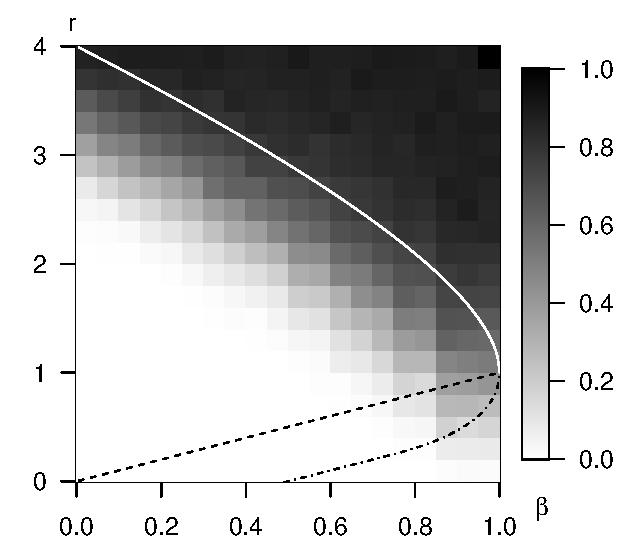
\includegraphics[width=0.4\textwidth]{./figures/simulated_phase_diagram_p100.eps}
      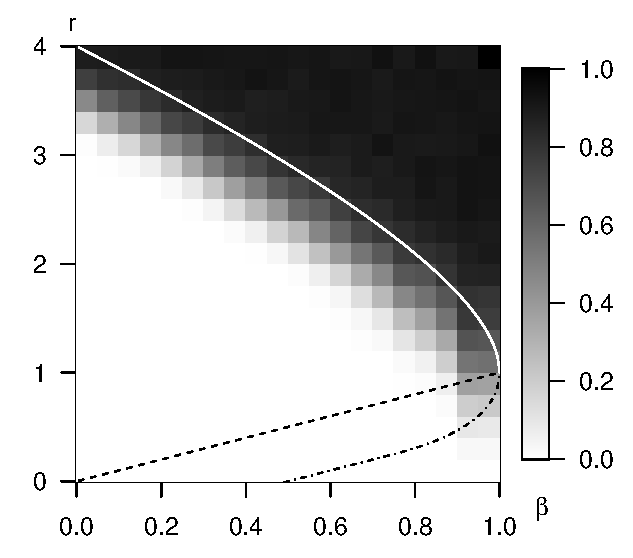
\includegraphics[width=0.4\textwidth]{./figures/simulated_phase_diagram_p10000.eps}
      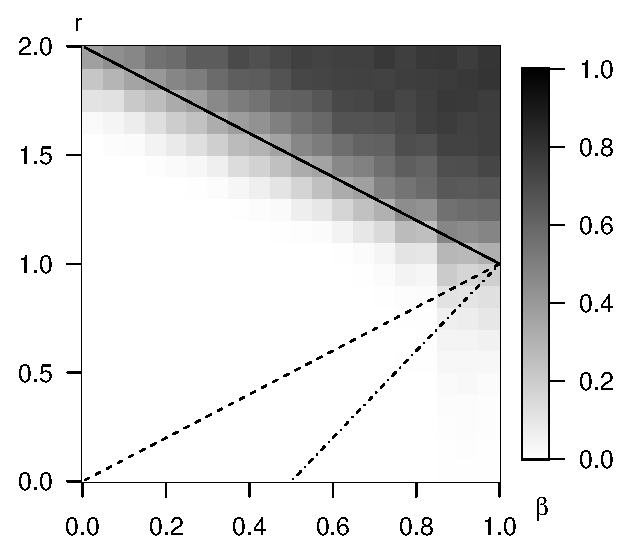
\includegraphics[width=0.4\textwidth]{./figures/simulated_phase_diagram_Laplace_p100_4.eps}
      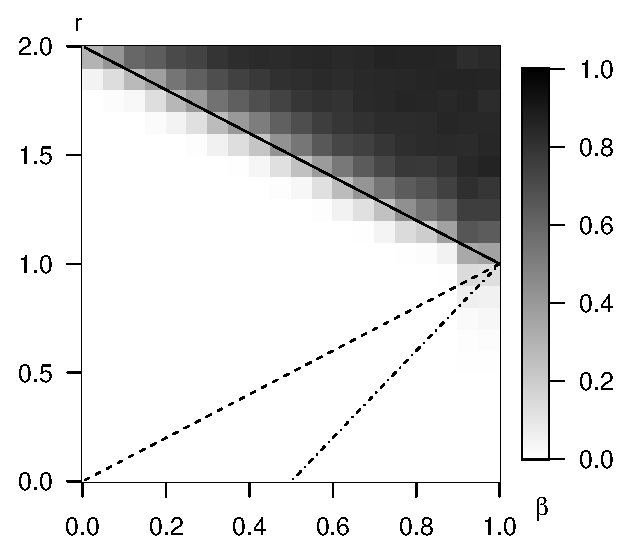
\includegraphics[width=0.4\textwidth]{./figures/simulated_phase_diagram_Laplace_p10000_4.eps}
      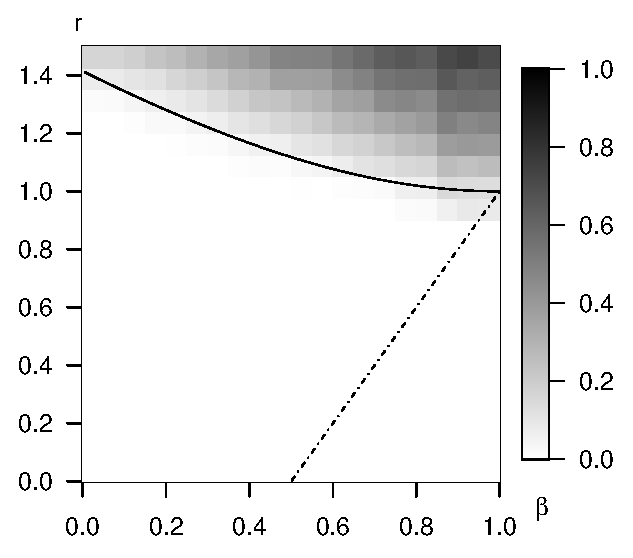
\includegraphics[width=0.4\textwidth]{./figures/simulated_phase_diagram_NLC_p100.eps}
      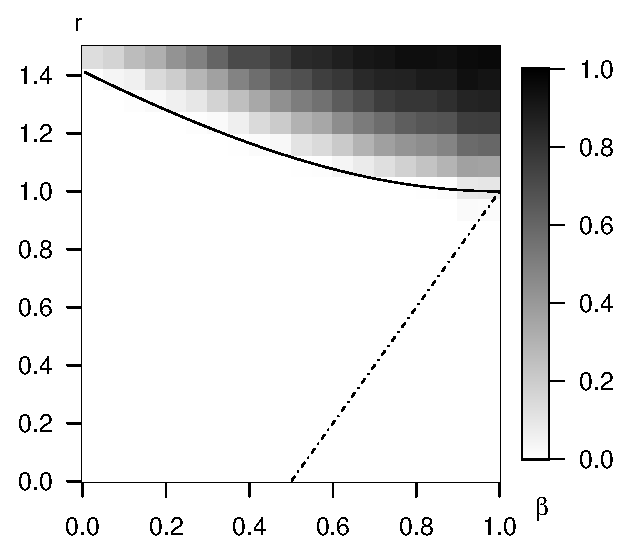
\includegraphics[width=0.4\textwidth]{./figures/simulated_phase_diagram_NLC_p10000.eps}
      \caption{The empirical probability of exact support recovery from numerical experiments, as a function of sparsity level $\beta$ and signal sizes $r$, 
      from Gaussian error models (upper panels), Laplace error models (middle panels), and generalized Gaussian with $\nu=1/2$ (lower panels); darker color indicates higher probability of exact support recovery. 
      The experiments were repeated 1000 times for each sparsity-signal size combination, and for dimensions $p=100$ (left panels) and $p=10000$ (right panels). 
      The numerical results agree with the boundaries described in Theorem \ref{thm:sufficient}. The convergence is noticeably slower for under the heavier 
      generalized Gaussian ($\nu=1/2$) errors.  For reference, the dashed and dash-dotted lines represent the weak classification and detection boundaries
       (see Chapter \ref{chap:phase-transitions}).
      \label{fig:phase-simulated}}
\end{figure}

